\section{Das Das Rosenblatt-Perzeptron}


\subsection{Cells that fire together, wire together: Synaptische Plastizität}

Donald Hebb (1904 - 1985), gebürtiger Kanadier, Sohn eines Ärzte-Elternpaares und 1965 nominiert für den Nobelpreis [BM03:1014], geht als junger Mann einer Karriere als Schriftsteller nach.
Er studiert Englisch als Hauptfach und macht 1924 seinen Bachelor\footnotemark[1] [Coo05:852], doch die Schriften Freuds, mit denen er sich nach seinem Abschluss beschäftigt, wecken in ihm den Wunsch, sich tiefer mit Psychologie zu beschäftigen [BM03 S. 1013]: An der McGill Universität in Montreal\footnotemark[2] macht er 1932 seinen Master darin\footnotemark[3], und leitet dort 16 Jahre später als Professor die Fakultät für Psychologie [Coo05:853].

\footnotetext[1]{
    an der Dalhousie Universität: https://dal.ca (abgerufen 17.08.2023)
}
\footnotetext[2]{
    McGillUniversität, Montreal, Quebec (Kanada): https://www.mcgill.ca/neuro/about/donald-hebb-phd (abgerufen 16.08.2023)
}
\footnotetext[3]{
    zu der Zeit studierte er in Teilzeit an der McGill Universität: ``as a part time graduate student`` [Kle99:1]. Seine Master-Arbeit schrieb er aufgrund einer Erkrankung im Bett [BM03:1014]
}


Seine Faszination darüber, wie das Gehirn lernt, Informationen verarbeitet und speichert [Str01:298 ff.] wird Bestandteil seiner Forschungsarbeit: 1949 veröffentlicht er das Buch ``\textbf{The organization of Behavior: A Neuropsychological Theory}`` [Heb49]; seine darin formulierten Postulate\footnotemark[4] [Kle99:2 f.] liefern einen wichtigen Beitrag für die Neurowissenschaften\footnotemark[5].
Oft zitiert wird seine Idee bzgl. synaptischer Verstärkung, was heute als \textbf{Hebbsche Synapse} bekannt ist [AR88:4, Abs. 5]\footnotemark[6]:

\blockquote[{[Heb88:50, Hervorhebung i.O.]}]{
    \textit{When an axion of cell} A \textit{is near enough to excite a cell} B \textit{and repeatedly or persistently takes part in firing it, some growth process or metabolic change takes place in one or both cells such that} A\textit{'s efficiency, as one of the cells firing} B\textit{, is increased.}
}

\footnotetext[4]{
    es sind ``three pivotal postulates`` {[Kle99:2 f.]}
}
\footnotetext[5]{
als hätte sein Buch eine Art Golgräberstimmung in der der Psychologie ausgelöst, schreibt [Kle99] ``It attracted many
brilliant scientists into psychology, made McGill University a North American mecca for scientists interested in brain mechanisms of behaviour, led to many important discoveries, and steered contemporary psychology onto a more fruitful path.`` [Kle99:1]
}
\footnotetext[6]{
    sowie als Zitat: \textit{a:} ``[...] any two cells or systems of cells that are repeatedly active at the same time will tend to become “associated,” so that activity in one facilitates activity in the other.`` [Heb88:52, ``Mode of perceptual Integration: The Cell-Assembly``] sowie \textit{b:} ``A series of such events [Aktivierung von ``cell-assemblies``] constitutes a “phase sequence”—the thought process. [Heb88:48, ``Mode of perceptual Integration: The Cell-Assembly]; die Aussage findet sich im Original [Heb49] bereits in ``Introduction``:xi-xix
}


Derartige Veränderungen synaptischer Verbindungen wird als \textbf{Hebbsche Lernregel} [BCP18:985, ``Hebb'sches Lernen``] bezeichnet.
Das damit verbundene geflügelte Wort \textit{Cells that fire together, wire together}\footnotemark[7] beschreibt die Hypothese bildhaft.
Seine Idee der ``\textbf{Cell Assembly}`` (siehe \footnotemark[6], Zitat \textit{b}) schließt daran an: Damit sind Verbände von Neuronen gemeint, die miteinander verschaltet sind, und deren Verbindungen durch das Hebbsche Lernen so sehr verstärkt sind, das die Aktivierung einzelner Zellen in diesen Verbänden ausreicht, das alle Zellen aktiviert werden [BCP18:907-908, ``Hebb und der Neuronenverband``].


Hebbs Theorien gelten durch die Forschung als bestätigt\footnotemark[8], und mit der von Hebb formulierten synaptische Plastizität wurde auch eine Idee für lernende künstliche neuronale Netze geliefert\footnotemark[9].
In Abschnitt~\ref{mcp-summary} haben wir geschlossen, dass ein MCP-Netz nur durch vorhergehende Analyse der Aufgabe und Anpassung der Topologie von Außen zur Lösung einer Aufgabe imstande ist.
Hebbs Erkenntnis führt kurz vor Beginn der 60er Jahre zu einem Modell, das in der Lage ist, sich selbst anzupassen.

\footnotetext[7]{
    Zumindest in [Heb49] findet sich kein solches Zitat. [KG14:2] behauptet: ``This mnemonic phrase was first introduced by Carla Shatz [12] in an article for the Scientific American aimed at lay public`` und meint damit den Satz ``In a sense, then, cells that fire together wire together.`` in [Sha92:94]. {https://en.wikipedia.org/wiki/Hebbian{\_}theory{\#}cite{\_}ref-2} (abgerufen 16.08.2023) hingegen schreibt den Ursprung [LS92] zu: ``neurons wire together if they fire together.`` [LS92:211]
}


\footnotetext[8]{
    vgl. [BLS19:833, Abs. 2 f.], außerdem [YLC+14] und [BL73]. [BPC18:875, Exkurs 23.5] verweist auf [Cop78]
}
\footnotetext[9]{
    ``[Hebb] laid the foundation for neoconnectionism which seeks to explain cognitive processes in terms of connections between assemblies of real or artificial neurons.`` [Kle99:2]
}


\subsection{Das Perzeptron - ein linearer Klassifizierer}

Bereits 1954 wurden Versuche unternommen, lernfähige neuronale Netze zu modellieren [Ros62:24, Abs. 2]\footnotemark[10].
Erst 1958 schafft es ein Modell, eine Sensation\footnotemark[11] auszulösen: Das \textbf{Perceptron} (im folgenden ``Perzeptron``) [AR88:90]\footnotemark[12].
1957 beschreibt es sein Schöpfer Frank Rosenblatt (1928 - 1971) in [Ros57] als Teil eines internen Forschungsprojektes des \textit{Cornell Aeronautical Labors}: Die Forschungseinrichtung gehörte von 1946 bis 1972\footnotemark[13] zu der Cornell Universität\footnotemark[14], an der Rosenblatt 1950 seinen A.B und 1956 seinen Ph.D. gemacht hatte, und an der er bis zu seinem Lebensende\footnotemark[15] als Psychologe und Neurobiologe forschen und lehren wird [Ehb71].

\footnotetext[10]{
    Rosenblatt verweist hier auf [CF54]
}
\footnotetext[11]{
    In der Presse publikumswirksam, aber wenig vertrauenserweckend: ``Frankenstein Monster Designed by Navy Robot That Thinks`` [Ros62:v]. Vgl. dazu aktuelle Schlagzeilen der hiesigen Boulevardpresse zum Thema KI. bild.de titelt: ``Übernehmen Computer die Weltherrschaft?`` (https://www.bild.de/news/ausland/news-ausland/experten-warnen-ki-so-gefaehrlich-wie-pandemien-und-atomkrieg-84130180.bild.html, abgerufen 27.08.2023) als Reaktion auf ``Statement on AI Risk`` des \textit{Center for AI Safety}, in dem zahlreiche Wissenschaftler zur Vorsicht beim Umgang, Einsatz und Forschung von KI mahnen. Im Wortlaut: ``Mitigating the risk of extinction from AI should be a global priority alongside other societal-scale risks such as pandemics and nuclear war.`` (https://www.safe.ai/statement-on-ai-risk, abgerufen 27.08.2023)
}
\footnotetext[12]{
vgl. auch [MP69:xix] ``Interest in connectionist networks revivied dramatically in 1962 with the publication of Frank Rosenblatt's book \textit{Principles of Neurodynamics}, [...]`` (Hervorhebung i.O.)
}
\footnotetext[13]{
    Seit 1972 Calspan Corporation [BB06], https://calspan.com/ (abgerufen 18.08.2023)
}
\footnotetext[14]{
    https://www.cornell.edu/, abgerufen 18.08.2023

}
\footnotetext[15]{
    1971 durch einen Bootsunfall [Car71]
}

\subsection*{The Perceptron - A perceiving and recognizing automaton}
Das Forschungsprojekt ``\textit{Perceiving and Recognizing Automaton}`` beschreibt einen Apparat, der mittels einer Kamera geometrische Figuren erkennen und zuordnen kann.
Die Funktionen simuliert Rosenblatt zunächst auf einem IBM 704 Rechner [Ros60], bevor  die Hardware Anfang der 60er Jahre als \textit{Mark 1 Perceptron} gebaut wird: 400 Cadmiumsulfid-Photozellen auf einem 20x20 großen Raster angeordnet - dem \textbf{S-System} (\textbf{S} = \textit{Sensory}) - leiten Signale an das \textbf{A-System} (\textbf{A} = \textit{Association}); dort werden sie registriert und ausgewertet, und schlussendlich über das \textbf{R-System} (\textbf{R} = \textit{Response}) ausgegeben (vgl. [Ros57:4, f.], [Ros58 S. 389 ff.] sowie [Bis06:193 ``Frank Rosenblatt`` sowie S. 196 Figure 4.8]).
Dabei lernt die Maschine im ersten Schritt durch die Unterstützung der Ingenieure, wie gegebene Formen zu interpretieren sind: Für aktivierte Photozellen wird die erwartete Ausgabe manuell festgelegt.
Die Verbindungen zwischen den \textbf{S}-, \textbf{A}- und \textbf{R}-Units erinnert nicht nur von der Namensgebung her an biologische Neuronen, auch deren Struktur und Verschaltung wird hier als Vorbild genommen\footnotemark[16] [Ros62:4, Abs. 2].


\footnotetext[16]{
    Die \textbf{S}-Units konnten sowohl hemmende als auch erregende Signale in das \textbf{A}-System einspeisen. Darüber hinaus war das \textbf{R}-System in der Lage, über Rückkoppelungen hemmende Signale an das \textbf{A}-System zu senden: Damit sollte verhindert werden, dass weitere \textbf{R}-Units aktiviert werden, die sich mit den bereits aktivierten Units gegenseitig ausschließen. [Ros57:4, Punkt (3)]
}

\begin{figure}[h]
    \centering
    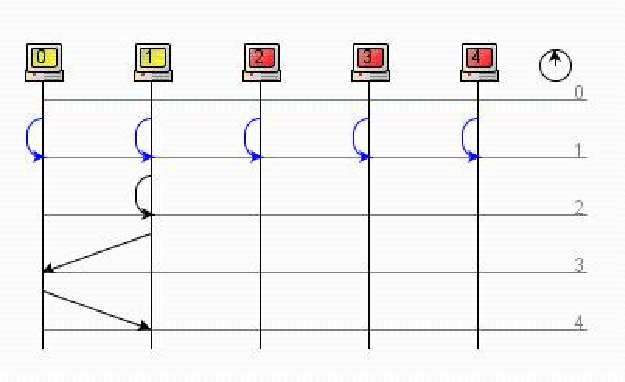
\includegraphics{images/p1ReadSeq.pdf}
    \caption{Schematische Darstellung der S, A, R Units}
    \label{fig-sarunits}
\end{figure}

\subsection{Das Modell}

Rosenblatt definiert das Perzeptron wie folgt\footnotemark[17]:

\footnotetext[17]{
    Definitionen aller Zustände, Signale und Funktionen in [Ros62:79 - 94]
}


\blockquote[{[Ros62:83, ``DEFINITION 17`` (Hervorhebung i.O.)]}]{
    A \underline{perceptron} is a network of S, A, and R units with a variable interaction matrix \textit{V} which depends on the
    sequence of past activity states of the network.
}

Für die \textbf{A}-Units wird definiert:

\blockquote[{[Ros62:81, ``DEFINITION 9`` (Hervorhebung i.O.)]}]{
    A \underline{simple A-unit} is a logical decision element, which
    generates an output signal if the algebraic sum of its
    input signals, $\alpha_i$ , is equal or greater than a threshold
    quantity, $\Theta > 0$. The output signal $a^*_i$ is equal to $+1$ if $\alpha_i \geq \Theta$ and $0$ otherwise. If $a^*_i = +1$,
    the unit is said to be \underline{active}.
}


Ähnlichkeiten zu der inAbschnitt~\ref{mcp-inputactivfunc} beschriebenen Aktivierungsfunktion sind durchaus erkennbar.
Rosenblatt selber weist darauf hin, dass er sein Modell direkt von dem von McCulloch und Pitts eingeführten Modell ableitet\footnotemark[18]. Darüber hinaus weist er auch auf Einflüsse von Hebb und von Neumann hin [Ros62:5].\\

\footnotetext[18]{
    vgl. auch ``Ein \texit{einfaches Perzeptron} ist eine McCulloch-Pitts-Zelle, die ihre Eingabe gewichtet berechnet.`` in [Roj93:57, ``Definition 3.1``, Hervorhebungen i.O.]
}

Das klassische Rosenblatt-Perzeptron verwendet in einem Netz von Eingabe- und Ausgabe-Knoten gewichtete Verbindungen - die Knoten selber sind Schwellenwertelemente, Verbindungen werden stochastisch ermittelt [Roj93:51, Abs. 3].
Nach Rosenblatts Veröffentlichung wurde sein Modell analysiert und verfeinert [Roj93:51, Abs. 3] u. a. von Minsky und Papert in [MP17], die wie folgt definieren:

\blockquote[{[MP17:12 (Herorhebung i.O.)]}]{
    A \underline{perceptron} is a device capable of computing all predicates which are linear in some given set $\Phi$ of partial predicates.
}


Prädikate sind hier Verbindungen zu den Eingabesignalen, die einen Wahrheitswert $0$ oder $1$ basierend auf der Eingabe $X$ berechnen.
Die Ausgabe der Prädikate werden individuell gewichtet und an die Zelle weitergeleitet, die die Aktivierungsfunktion implementiert (vgl. [Roj93:52] und [MP17:8-12]).


\begin{figure}[h]
    \centering
    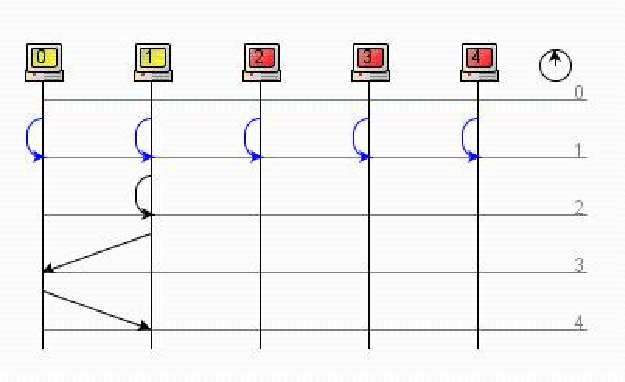
\includegraphics{images/p1ReadSeq.pdf}
    \caption{Schematische Darstellung der Eingabesignale, Prädikate, Gewichte und Schwellenwertzelle [Ro93:53]}
    \label{fig-perctheda}
\end{figure}


Die Eingabefunktion setzt sich dann wie Gleichung~\ref{eq:gl-mcpinpfunc} aus der Summe der Produkte der Prädikate $P_i \in \Phi$ (wobei $P_i(X) \in \{0, 1\}$) und den Gewichten $w_i \in \R$ der Verbindungen zusammen (s. Gleichung~\ref{eq:gl-rpinput}), und die Aktivierungsfunktion (s. Gleichung~\ref{eq:gl-rpact}) ist wieder eine Treppenfunktion mit dem reellen Schwellenwert $\Theta$:

\begin{equation}
g:= g(X) = \sum^n_{i=1} P_i(X) w_i
\label{eq:gl-rpinput}
\end{equation}

\begin{equation}
    f:= f(x) = f(g(X)) = \begin{cases}
                          1 \text{ falls } x >= \Theta \\
                          0 \text{ falls } x < \Theta
\end{cases}
\label{eq:gl-rpact}
\end{equation}

\noindent
\textit{Minsky und Papert} weisen in ihrer Definition des Perzeptrons auf eine besondere Voraussetzung hin, die Thema des nächsten Abschnitts wird.

\subsection{Lineare Trennbarkeit}
Mit Gleichung~\ref{eq:gl-rpact} folgt für eine Eingabe, dass sie entweder eine $0$ oder $1$ als Ausgabe erzeugt.
Wir haben es hier also wieder mit einem binären Wertebereich zu tun, den wir auch als zwei unterschiedliche Klassen [RN09:812, Abs. 2] verstehen können: Eingabedaten können somit einer der beiden Klassen zugeordnet werden.
Im Folgenden wollen wir die Zusammenhänge geometrisch darstellen.
Der Einfachheit halber beschränken wir uns hierzu auf den zweidimensionalen Raum $\R_+^2$ und betrachten hier die \textit{1. Winkelhalbierende} im 1. Quadrant des kartesischen Koordinatensystems.
Die zugehörige \textit{Gerade} $L$ [Fis19:18] ist

\begin{equation}
L = \{(x_1, x_2) \in \R_+^2: x_1 = x_2\}
\end{equation}


\begin{figure}[h]
    \centering
    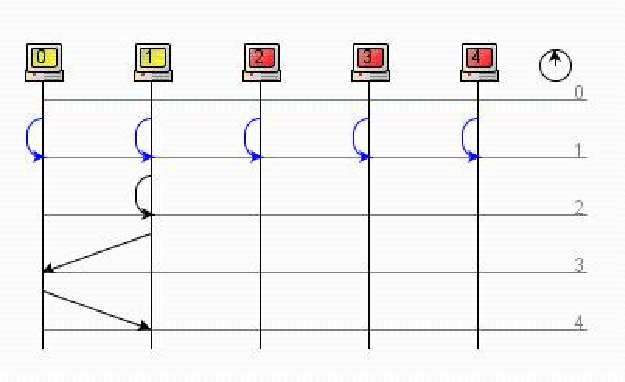
\includegraphics{images/p1ReadSeq.pdf}
    \caption{Winkelhalbierende im kartesischen Koordinatensystem}
    \label{fig-winkelhalbierende}
\end{figure}

Für beliebige Punkte $(x_1, x_2) \in \R_+^2$ gilt offensichtlich

\begin{equation}
x_1 - x_2 \begin{cases}
               > 0 \text{ falls } x_1 > x_2 \\
               = 0 \text{ falls } x_1 = x_2 \\
               < 0 \text{ falls } x_1 < x_2
\end{cases}
\end{equation}

Die \textit{Gerade} $L$ repräsentiert eine \textit{Hyperebene} [BHW+12 S. 81, ``Definition 2.3``] in $\R_+^2$.
Punkte, die nicht zu dieser Hyperebene gehören, liegen in dem Fall $\R_+^2$ in zwei unterschiedlichen \textit{Halbräumen}\footnotemark[19].
Die Halbräume und deren Trennung wird greifbarer durch die geometrische Darstellung in Abbildung~\ref{fig-halbraeume}.
Wir können feststellen, dass


\begin{itemize}
    \item Punkte, die $x_1 - x_2 > 0$ erfüllen (im folgenden $M_-$) in dem Halbrum \textit{unter} der durch $L$ beschriebenen Gerade liegen
    \item Punkte, für die  $x_1 - x_2 < 0$ gilt (im folgenden $M_+$) \textit{über} der durch $L$ beschriebenen Gerade liegen
    \item Punkte mit $x_1 - x_2 = 0$ \textit{auf} der Geraden liegen (im folgenden $\subset M_-$\footnotemark[20])
\end{itemize}


\begin{figure}[h]
    \centering
    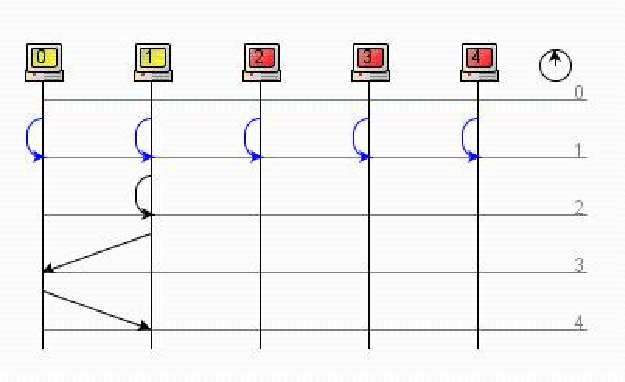
\includegraphics{images/p1ReadSeq.pdf}
    \caption{Skizzierung der durch die 1. Winkelhalbierende entstandenen Halbräume. Die Mengen $M_-$ und $M_+$ sind linear separierbar, die Gleichung für die \textit{Trenngerade} hierzu lautet $x_1 - x_2 = 0$}
    \label{fig-halbraeume}
\end{figure}

\footnotetext[19]{
    Renze, John; Uznanski, Dan; and Weisstein, Eric W. ``Half-Plane.`` From MathWorld--A Wolfram Web Resource. https://mathworld.wolfram.com/Half-Plane.html (abgerufen 21.08.2023)
}


\footnotetext[20]{
    Wenn die Hyperebene selbst im Halbraum enthalten ist, spricht man von einem _abgeschlossenen Halbraum_. (https://de.wikipedia.org/wiki/Halbraum, abgerufen 22.08.2023)
}


Formal ausgedrückt bedeutet das, dass $M_+$ und $M_-$ \textit{linear separabel} sind. Nach [Roj93] lautet die Definition für \textit{Lineare Trennbarkeit}:

\begin{definition}\footnotemark[21]

Zwei Mengen \textit{A} und \textit{B} von Punkten in einem \textit{n}-dimensionalen Raum sind \textit{linear trennbar}, falls \textit{n}+1 reelle Zahlen $w_1, ... , w_{n+1}$ existieren, so daß für jeden Punkt $x_1, ... , x_n \in A$ gilt

\begin{equation}
\sum^n_{i=1} w_ix_i \geq w_{n+1}
\label{eq:gl-defhalbraum-gl1}
\end{equation}

und für jeden Punkt $x_1, ... , x_n \in B$

\begin{equation}
    \sum^n_{i=1} w_ix_i < w_{n+1}
\label{eq:gl-defhalbraum-gl2}
\end{equation}
\label{def-halbraum}
\end{definition}

\footnotetext[21]{
    [Roj93:61, ``Definition 3.2``, Hervorhebungen i.O., Nummerierung eigene]
}


\noindent
Für unser Beispiel mit den oben eingeführten Mengen $M_- = \{(x_1, x_2) \in  \mathbb{R}_+^2: x_1 \geq x_2\}$ und $M_+=\{(x_1, x_2) \in  \mathbb{R}_+^2: x_1 < x_2\}$ in $ \mathbb{R}_+^2$ wählen wir $w_1 = -1, w_2 = 1, w_3 = 0$.
Dass diese Mengen nach Definition~\ref{def-halbraum} linear separabel sind, lässt sich leicht anhand einer Fallunterscheidung nachweisen:

\begin{enumerate}
    \item Fall $x_1 = x_2$: Es gilt $w_1x_1 + w_2x_2 = w_1x_1 + w_2x_1 = -x_1 + x_1 = w_3 = 0$. Mit $0 \geq 0$ ist somit Gleichung~\ref{eq:gl-defhalbraum-gl1} erfüllt.
    \item Fall $x_1 < x_2$: Es gilt $w_1x_1 = -x_1$. Addition von $w_1x_1$ auf beiden Seiten von $x_2 > x_1$ liefert $x_2 + (-x_1) = w_2x_2 + w_1x_1 > 0 = w_3$ und erfüllt Gleichung~\ref{eq:gl-defhalbraum-gl1}.
    \item Fall $x_1 > x_2$: Es gilt wieder $w_1x_1 = -x_1$. Addition auf beiden Seiten von $x_1 > x_2$ liefert $w_3 = 0 > x_2 + (-x_1) = w_2x_2 + w_1x_1$ und erfüllt Gleichung~\ref{eq:gl-defhalbraum-gl2}.
\end{enumerate}


\noindent
Die von \textit{Ertel} formulierte Definition\footnotemark[22] für ein Perzeptron wollen wir für die weiteren Betrachtungen übernehmen:

\footnotetext[22]{
    [Ert21:212, ``Definition 8.3``, Hervorhebungen i.O.]
}

\begin{definition}
\noindent
Sei $w = (w_1, ..., w_n) \in  \mathbb{R}^n$ ein Gewichtsvektor und $x \in  \mathbb{R}^n$ ein Eingabevektor. Ein \textbf{Perzeptron} stellt eine Funktion $P:  \mathbb{R}^n \to \{0, 1\}$ mit

\begin{equation}
P(x) = \begin{cases}
            1 \text{ falls } wx = \sum^n_{i=1} w_ix_i >0 \\
            0 \text{sonst}
\end{cases}
\end{equation}
\noindent
dar.

\end{definition}

\subsection{Die Lernregel}

Die Eigenschaft linearer Trennbarkeit von Daten ist eine wesentliche Voraussetzung dafür, dass ein Perzeptron \textit{konvergiert}: Die \textit{Lernregel} des Perzeptrons passt während der Laufzeit die Gewichte $w_1 ... w_n$ solange an, bis sie - eingesetzt in eine lineare Gleichung [Ert21:311] - die $n$-dimensionalen Daten entsprechend Definition~\ref{eq:gl-rpact} \textit{klassifizieren} kann.
Aus diesem Grund wird das Perzeptron auch \textbf{linearer Klassifizierer} genannt [Ert21:210 - 216].

Das Perzeptron \textbf{lernt} diese Gewichte zunächst durch \textit{Traningsdaten}\footnotemark[23].
Jeder Eintrag dieser Trainingsdaten ist einer erwarteten Ausgabe zugeordnet. Der Algorithmus besteht aus folgenden Schritten (vgl. [RM87 S. 65] sowie [RN09 S. 842]):


\footnotetext[23]{
    ``supervised learning``: überwachtes lernen; vgl. [RN09:811, ``18.2 Überwachtes Lernen``] sowie [Fau94:15]. \textit{Arbib et al.} weisen darauf hin, dass \textit{überwachtes Lernen} mit dem Perzeptron eingeführt wurde: ``Supervised learning adjusts the weights in an attempt to respond to explicit error signals provided by a “teacher,” which
    may be external, or another network in the same “brain.” This model was introduced in the perceptron model, [...].``  [Arb02:30, rechte Spalte unten]
}

\begin{enumerate}
    \item Wähle einen Datensatz und berechne die Ausgabe
    \item Wenn die Ausgabe $1$ ist, obwohl sie $0$ sein sollte (Fehler\footnotemark[24] $=-1$), verringere die Gewichte
    \item Wenn die Ausgabe $0$ ist, obwohl sie $1$ sein sollte  (Fehler $=1$), erhöhe die Gewichte
    \item Wenn die Ausgabe korrekt ist, passe die Gewichte nicht an
\end{enumerate}

\noindent
Die Beziehung zu der Hebbschen Lernregel formulieren \textit{Arbib et al.}\footnotemark[25]:

\footnotetext[24]{
    Der \textbf{Fehler} ist hierbei die Differenz von $\text{erwartete Ausgabe}$ und $\text{tatsächliche Ausgabe}$.
}

\footnotetext[25]{
    vgl. hierzu auch _Rosenblatt_ : ``[ein Perzeptron hat] a tendency to develop 'cell assemblies' (in Hebb's sense), and these cell-assemblies tend to rival one another for dominance at all times. [Ros62:464, Abs. 2, Anführungszeichen doppelt i.O.]
}


\blockquote[{[Arb03:20, rechte Spalte, Abs.1]}]{
    The best-known perceptron learning rule strengthens an active synapse if the efferent neuron fails to fire when it should have fired, and weakens an active synapse if the neuron fires when it should not have done so.
}

\noindent
Die Schritte werden so lange durchlaufen, bis für alle Trainingsdaten die Ausgabe korrekt ist, oder eine maximale Anzahl von Trainingsläufen erreicht wurde. 
Einen Trainingslauf nennt man dabei \textit{Epoche} [Fau94:436, ``Training epoch``]. 
Sind die Trainingsdaten linear separabel, \textit{konvergiert}\footnotemark[26] das Perzeptron nach einer endlichen Zahl von Epochen [MP17:164]\footnotemark[27], und ist danach in der Lage zu \textit{generalisieren} [Ert21:202].\\

\footnotetext[26]{
    ``iterative training processes converge if the weight updates reach equilibrium (stop changing)`` [Fau94:425, ``Convergence``]
}
\footnotetext[27]{
    Das Konvergenz-Theorem besagt: ``if a linear separation exists, the perceptron error-correction scheme will find it.`` [Arb03:20, ``Network Complexity``] Beweise führen [Ros62:111 ff.], [MP17:167 ff.] sowie [Nov62].
}

Da wir in unserem Beispiel nur Daten betrachtet haben, die durch eine Gerade durch den Ursprung ($(0,0)$) getrennt sind, brauchen wir noch eine Möglichkeit, die $x_2$-Koordinate der Trenngerade anzupassen.


\begin{figure}[h]
    \centering
    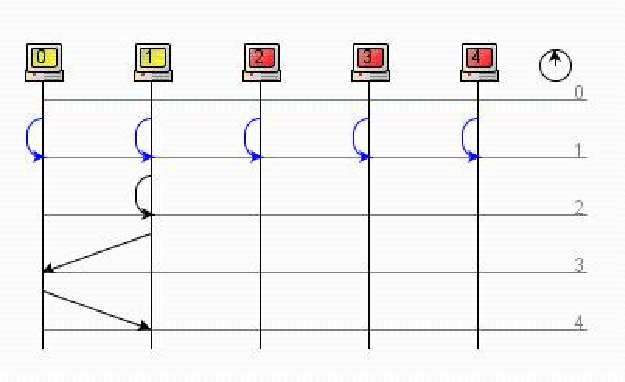
\includegraphics{images/p1ReadSeq.pdf}
    \caption{Daten, die nicht durch eine Ursprungsgerade separabel sind.}
    \label{fig-nichtseparierbar}
\end{figure}

\noindent
Dies erreicht man mit einer sogenannten \textbf{bias unit}. 
Das Bias-Gewicht\footnotemark[28] ist ein Wert, der zu der Gleichung aus Definition\ref{eq:gl-rpact} hinzuaddiert wird, und für eine Verschiebung der Ursprungsgeraden\footnotemark[29] sorgt.

\footnotetext[28]{
    vgl. [RN09:839]
}
\footnotetext[29]{
    im $ \mathbb{R}^n$ durch eine Hyperebene im Ursprung [Ert21:215]
}

Den Eingabedaten wird ein fester Eingabewert $x_{n+1} = 1$ hinzufügt: Der Eingabevektor $x \in  \mathbb{R}^n$ wird \textit{erweitert}: $(x_1, ..., x_n, 1)$ [Roj93:58, ``3.2.2 Gewichtete Netze mit einem kanonischen Baustein``].

\noindent
Der bias $b$ wird für unser Beispiel im $ \mathbb{R}^2$ mit Definition\ref{eq:gl-rpact} in die Berechnung Schwellenwerts miteinbezogen:

\begin{equation}
P(x) = \begin{cases}
            1 &\text{falls} &wx > 0 \\
            0 &\text{sonst}
\end{cases}
\end{equation}

\noindent
wobei

\begin{equation}
wx = b + \sum^n_{i=1} w_ix_i
\label{eq:gl-net}
\end{equation}

\noindent
Die Gleichung für die Trenngerade für unser Beispiel im $\mathbb{R}^2$ lautet somit

\begin{equation}
b + w_1x_1 + w_2x_2 = 0
\end{equation}

\noindent
Wenn wir $b$ auf die rechte Seite der Gleichung bringen, kann $b$ auch als Schwellenwert $\Theta = -b$ betrachtet werden:

\begin{equation}
w_1x_1 + w_2x_2 = \Theta
\end{equation}

\noindent
Für unser $x_2$ im $ \mathbb{R}^2$ folgt dann insgesamt mit $w_2 = 1$ und $x_1 = 0$:

\begin{equation}
x_2 = \Theta/w_2 -(w_1/w_2)x_1  = \Theta
\end{equation}

\noindent
was der Abstand $x_2$ von der $y$-Achse ist.

\noindent
Mit $b$ als Teil der Eingabe folgt auch dessen Gewichtung $bw_{n+1} = w_{n+1}$.
Mit $0$ als Schwellenwert wird dadurch eine Verschiebung der Trenngeraden entlang der $y$-Achse im $ \mathbb{R}^2$ bzw. eine Verschiebung der Hyperebene im $ \mathbb{R}^n$ ermöglicht[Ert21:215] \footnotemark[30].

\begin{figure}[h]
    \centering
    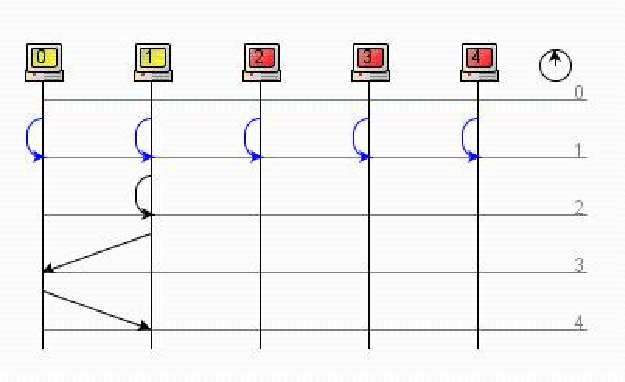
\includegraphics{images/p1ReadSeq.pdf}
    \caption{Geometrische Interpretation der Perzeptron-Funktion im $\mathbb{R}^2$}
    \label{fig-geominterpretation}
\end{figure}


\subsection*{Lernrate}
Bevor wir uns eine Implementierung in Python anschauen, wollen wir noch kurz die \textbf{Lernrate} $\eta$ (in der Literatur auch $\alpha$) erklären.
Wie wir in diesem Abschnitt erfahren haben, berechnet die Lernregel die Gewichte auf Basis des \textit{Fehlers}, also der Differenz von $\text{erwartete Ausgabe}$ und $\text{tatsächliche Ausgabe}$: Ist der Fehler $-1$, werden die Gewichte verringert, ist der Fehler 1, werden die Gewichte erhöht.
Die Lernrate $\eta$ ist der Koeffizient für die Gewichtsanpassung \footnotemark[31].
Üblicherweise liegt $\eta$ zwischen $0$ und $1$\footnotemark[32] [Fau94:61].

\footnotetext[30]{
    ein hilfreicher Überblick über die geometrischen Zusammenhänge ist in ``Einführung in die Neuroinformatik`` von Prof. Dr. G. Sommer https://www.informatik.uni-kiel.de/inf/Sommer/doc/Downloads/Skripte/neuroskript.pdf:33 ff. zu finden (abgerufen 27.08.2023)
}
\footnotetext[31]{
    Auch \textit{Schrittweite}: vgl [GBC18:93] und [RN09:172]
}
\footnotetext[32]{
    ``$\alpha$ [$\eta$] ist eine kleine Konstante`` [RN09:172, Abs. 2]. Gleiche Stelle beleuchtet das Für und Wider kleiner und großer Werte von $\eta$; \textit{Salomon} weist in [Dor90:173] darauf hin, dass eine geeignete Lernrate auch von der Aufgabenstellung abhängt.
}


\subsection{Implementierung in Python}

Wie bereits Abschnitt~\ref{seq-mcpbool} wollen wir auch mit dem Rosenblatt Perzeptron boolesche Funktionen nachbilden.
Das folgende Beispiel bezieht sich auf die \textbf{AND}-Funktion (vgl. Tabelle~\ref{tab:and}).

Zunächst definieren wir zwei Mengen $M_+$ und $M_-$: Für Elemente in $M_+$ ist die erwartete Ausgabe $1$, für Elemente in $M_-$ ist sie $0$:

\begin{equation}
M_+ := \{(1, 1)\}\\
\end{equation}

\begin{equation}
M_- := \{(0, 0), (0,1), (1,0)\}
\end{equation}

\begin{figure}[h]
    \centering
    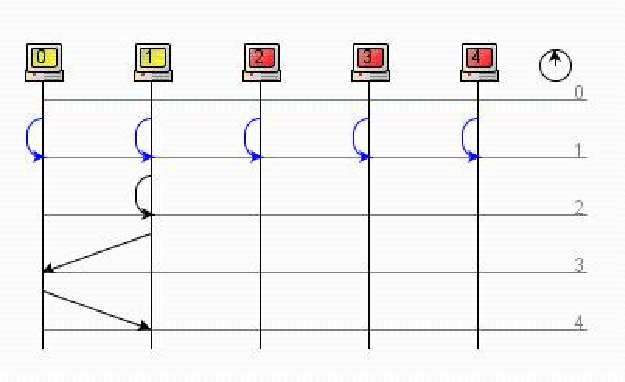
\includegraphics{images/p1ReadSeq.pdf}
    \caption{Geometrische Interpretation der Perzeptron-Funktion im $\mathbb{R}^2$}
    \label{fig-rpand}
    \small Die Abbildung zeigt alle möglichen zweiwertigem Interpretation von $A \land B$ in einem kartesischen Koordinatensystem. Offensichtlich ist die Anzahl der möglichen Trenngeraden mit $L \subset  \mathbb{R}^2$ unendlich.
\end{figure}

\pagebreak
Für unsere Perzeptron-Implementierung in Python\footnotemark[33] implementieren wir die Lernregel wie folgt:

\footnotetext[33]{
    vollständiger Quellcode unter https://github.com/ThorstenSuckow/pylabs (abgerufen 25.08.2023)
}

\begin{lstlisting}[language=Python]
    for epoch in range(epochs):

        errors = 0

        for i in range(n):
            expected = y[i]
            net = X[i] @ self.w + self.bias
            result = self.heaviside(net)
            error = 0

            if result != expected:
                error = expected - result

                self.w += (X[i] * learning_rate * error)
                self.bias += learning_rate * error
\end{lstlisting}

\noindent
Der Algorithmus erhält eine vorgegebene Zahl von Epochen, in denen wir eine vollständige Konvergenz erwarten.
Innerhalb einer Epoche werden alle \verb|n| Trainingsdaten (enthalten in \verb|X|) durchgegangen.
In \verb|y| finden wir die erwartete Klassifizierung der Trainingsdaten:
Ist \verb|X[i] = [1,1]|, entspricht \verb|y[i] = 1| (vgl. Gleichung~\ref{eq:gl-expnet}).
\verb|net| entspricht dem Ergebnis von Gleichung~\ref{eq:gl-net}, und das Ergebnis \verb|result| der \textbf{Heaviside}-Funktion mit

\begin{equation}
exp = \begin{cases}
           1 \text{ falls } \text{net} \geq 0 \\
           0 \text{ sonst}
\end{cases}
\label{eq:gl-expnet}
\end{equation}

\noindent
Die Lernregel wird so lange durchlaufen, bis für alle Trainingsdaten kein Fehler \verb|error| mehr auftritt oder alle Epochen ausgeschöpft sind.\\

\noindent
Der Algorithmus nutzt folgende Nomenklatur:\\


$\eta := 1 \space \space \text{ (Lernrate)}$

$b := 0 \space \space \text{ (Bias)}$\\

$w := \begin{pmatrix}
          1 \\
          1
\end{pmatrix}\space \space \text{ (Gewichtsvektor)}$
\\
\\

$M_+ := \{(1, 1)\}$

$M_- := \{(0, 0), (0,1), (1,0)\}$

$net = w_1x_1 + w_2x_2 + b$\\

$exp = \begin{cases}
           1 \text{ falls } (x_1, x_2) \in M_+ \\
           0 \text{ sonst }
\end{cases}  \space \space \text{ (erwartete Ausgabe)}$
\\
\\

$res =  \begin{cases}
            0 \text{ falls } net < 0 \\
            1 \text{ sonst }
\end{cases}  \space \space \text{ (berechnete Ausgabe)}$\\

$err = exp - res  \space \space \text{ (Fehler)}$

$w^u = w + (x_1, x_2) * \eta * err  \space \space \text{ (aktualisierter Gewichtsvektor)}$

$b^u = b + \eta * err \space \space \text{ (aktualisierter Bias)}$\\


\noindent
Mit der o.a. Implementierung konvergiert das Perzeptron innerhalb von 5 Epochen.
In jeder Epoche werden 4 einzelne Daten trainiert, was insgesamt einer Anzahl von 20 Trainingsschritten entspricht.
Das Perzeptron hat also für $w_1$, $w_2$ Werte gefunden, so dass die folgenden 4 Ungleichungen gleichzeitig erfüllt sind:\\



$w_10 + w_20 < \Theta$\\

$w_11 + w_20 < \Theta$\\

$w_10 + w_21 < \Theta$\\

$w_11 + w_21 \geq \Theta$\\



Die folgenden Tabellen zeigen die Anpassungen im Detail. 
Die geometrische Darstellung hierzu findet sich in Abbildung~\ref{fig-rp-and-epochs}.

\setlength{\tabcolsep}{0.8em}
\begin{table} %[hbtp]
    \centering
    \begin{tabular}{c | c | c | c | c | c | c | c | c | c | c | c | c}
        Epoche & $x_1$ & $x_2$ & $w_1$ & $w_2$ & $b$ & $net$ & $exp$ & $res$ & $err$ & $w^u_1$ & $w^u_2$ & $b^u$ \\
        \hline
        1.1& 0     & 0     & 1     & 1     & 0   & 0     & 0     & 1     & -1  & 1       & 1       & -1 \\
        1.2& 1     & 0     & 1     & 1     & -1  & 0     & 0     & 1     & -1  & 0       & 1       & -2 \\
        1.3& 0     & 1     & 0     & 1     & -2  & -1    & 0     & 0     & 0   & 0       & 1       & -2 \\
        1.4& 1     & 1     & 0     & 1     & -2  & -1    & 1     & 0     & 1   & 1       & 2       & -1 \\
    \end{tabular}
    \caption{Epoche 1 für \textbf{AND}}
    \label{tab:mcp-andep1}
\end{table}

\setlength{\tabcolsep}{0.8em}
\begin{table} %[hbtp]
    \centering
    \begin{tabular}{c | c | c | c | c | c | c | c | c | c | c | c | c}
        Epoche & $x_1$ & $x_2$ & $w_1$ & $w_2$ & $b$ & $net$ & $exp$ & $res$ & $err$ & $w^u_1$ & $w^u_2$ & $b^u$ \\
        \hline
        2.1& 0     & 0     & 1     & 2     & -1  & -1    & 0     & 0     & 0   & 1       & 2       & -1    \\
        2.2& 1     & 0     & 1     & 2     & -1  & 0     & 0     & 1     & -1  & 0       & 2       & -2    \\
        2.3& 0     & 1     & 0     & 2     & -2  & 0     & 0     & 1     & -1  & 0       & 1       & -3    \\
        2.4& 1     & 1     & 0     & 1     & -3  & -2    & 1     & 0     & 1   & 1       & 2       & -2    \\
    \end{tabular}
    \caption{Epoche 2 für \textbf{AND}}
    \label{tab:mcp-andep2}
\end{table}

\setlength{\tabcolsep}{0.8em}
\begin{table} %[hbtp]
    \centering
    \begin{tabular}{c | c | c | c | c | c | c | c | c | c | c | c | c}
        Epoche & $x_1$ & $x_2$ & $w_1$ & $w_2$ & $b$ & $net$ & $exp$ & $res$ & $err$ & $w^u_1$ & $w^u_2$ & $b^u$ \\
        \hline
        3.1& 0     & 0     & 1     & 2     & -2  & -2    & 0     & 0     & 0   & 1       & 2       & -2    \\
        3.2& 1     & 0     & 1     & 2     & -2  & -1    & 0     & 0     & 0   & 1       & 2       & -2    \\
        3.3& 0     & 1     & 1     & 2     & -2  & 0     & 0     & 1     & -1  & 1       & 1       & -3    \\
        3.4& 1     & 1     & 1     & 1     & -3  & -1    & 1     & 0     & 1   & 2       & 2       & -2    \\
    \end{tabular}
    \caption{Epoche 3 für \textbf{AND}}
    \label{tab:mcp-andep3}
\end{table}


\setlength{\tabcolsep}{0.8em}
\begin{table} %[hbtp]
    \centering
    \begin{tabular}{c | c | c | c | c | c | c | c | c | c | c | c | c}
        Epoche & $x_1$ & $x_2$ & $w_1$ & $w_2$ & $b$ & $net$ & $exp$ & $res$ & $err$ & $w^u_1$ & $w^u_2$ & $b^u$ \\
        \hline
        4.1& 0     & 0     & 2     & 2     & -2  & -2    & 0     & 0     & 0   & 2       & 2       & -2    \\
        4.2& 1     & 0     & 2     & 2     & -2  & 0     & 0     & 1     & -1  & 1       & 2       & -3    \\
        4.3& 0     & 1     & 1     & 2     & -3  & -1    & 0     & 0     & 0   & 1       & 2       & -3    \\
        4.4& 1     & 1     & 1     & 2     & -3  & 0     & 1     & 1     & 0   & 1       & 2       & -3    \\
    \end{tabular}
    \caption{Epoche 4 für \textbf{AND}}
    \label{tab:mcp-andep4}
\end{table}

\setlength{\tabcolsep}{0.8em}
\begin{table} %[hbtp]
    \centering
    \begin{tabular}{c | c | c | c | c | c | c | c | c | c | c | c | c}
        Epoche & $x_1$ & $x_2$ & $w_1$ & $w_2$ & $b$ & $net$ & $exp$ & $res$ & $err$ & $w^u_1$ & $w^u_2$ & $b^u$ \\
        \hline
        5.1& 0     & 0     & 1     & 2     & -3  & -3    & 0     & 0     & 0   & 1       & 2       & -3    \\
        5.2& 1     & 0     & 1     & 2     & -3  & -2    & 0     & 0     & 0   & 1       & 2       & -3    \\
        5.3& 0     & 1     & 1     & 2     & -3  & -1    & 0     & 0     & 0   & 1       & 2       & -3    \\
        5.4& 1     & 1     & 1     & 2     & -3  & 0     & 1     & 1     & 0   & 1       & 2       & -3    \\
    \end{tabular}
    \caption{Epoche 5 für \textbf{AND}}
    \label{tab:mcp-andep5}
\end{table}




\begin{figure}[h]
    \centering
    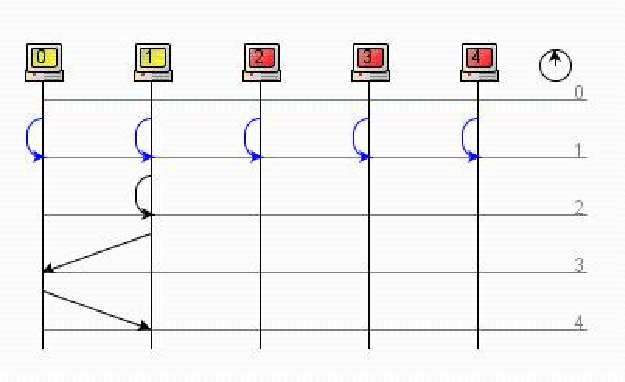
\includegraphics{images/p1ReadSeq.pdf}
    \caption{}
    \label{fig-rp-and-epochs}
    \small Ein vollständiger Lauf über 5 Epochen für die AND-Funktion. Blaue gestrichelt ist die Trenngerade, auf der senkrecht der Gewichtsvektor (orange) steht. Grün umrandete Punkte sind Ziel des Trainingsschrittes und bedingen den ``Änderungsvektor`` (schwarz), der die Anpassung von $w$ im nächsten Schritt angibt. (Quelle: eigene)
\end{figure}


\subsection{Die XOR-Funktion}

Wenn ein Perzeptron nicht konvergiert, kann es ausreichen, die Anzahl der Epochen zu erhöhen, damit ein passender Gewichtsvektor gefunden wird\footnotemark[34].

\footnotetext[34] {
    \textit{Arbib et al} berufen sich auf das Konvergenz-Theorem und führen an, dass ``[das Rosenblatt Perzeptron] does not yield an endless seesaw, but will eventually converge to a correct set of weights if one exists, albeit perhaps after many iterations through the set of trial patterns.`` [Arb03:20, rechte Spalte, Abs. 1]: \textit{Minsky und Papert} formulieren lose: ``if the sets are separable [...], then the program will separate them`` [MP17:165, Abs. 1] und stellen im Hinblick auf Parameteranpassungen fest: ``Usually, when a failure occurred, neither prolonging the training experiments nor building larger machines helped.`` [MP17:xix, Abs. 3]
}


\begin{figure}[h]
    \centering
    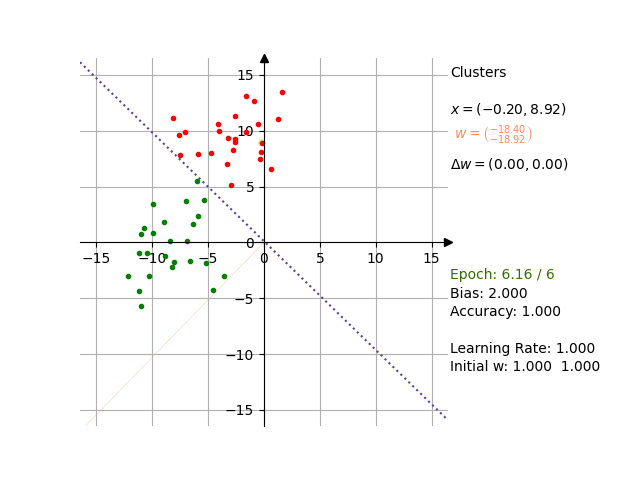
\includegraphics{images/rosenblatt/blob_success.png}
    \caption{}
    \label{fig-rp-blobs}
    \small Ein Perzeptron wird mit einer großen Datenmengen (50 Einträg) trainiert. Nach knapp 300 Trainingsschritten (in der 6ten Epoche) wird die Trenngerade gefunden. (Quelle: eigene)
\end{figure}

\noindent
Allerdings kann es bereits bei wenigen Daten und beliebig großer Epochenzahl passieren, dass ein Perzeptron nicht konvergiert, nämlich wenn die Daten nicht linear separabel sind [Arb03:2, rechte Spalte, Abs. 1].

Als Beispiel betrachten wir die boolesche Funktion \textbf{XOR} (vgl. Tabelle~\ref{tab:xor}). In Abbildung~\ref{fig-rp-xor } ist die geometrische Repräsentation der möglichen Interpretationen für $A \oplus B$ dargestellt.
Zwar lassen sich die Elemente separieren, aber nicht linear.
Es müßte sonst ein $w_1, w_2$ existieren, das folgende Ungleichungen erfüllt:\\


$w_10 + w_20 < \Theta$\\

$w_11 + w_20 \geq \Theta \implies w_1 \geq \Theta$\\

$w_10 + w_21 \geq \Theta \implies w_2 \geq \Theta$\\

$w_11 + w_21 < \Theta$\\

\noindent
Offensichtlich kann $w_1 + w_2 < \Theta$ nicht erfüllt werden, wenn gleichzeitig $w_1 \geq \Theta$ und $w_2 \geq \Theta$ gilt.

\begin{figure}[h]
    \centering
    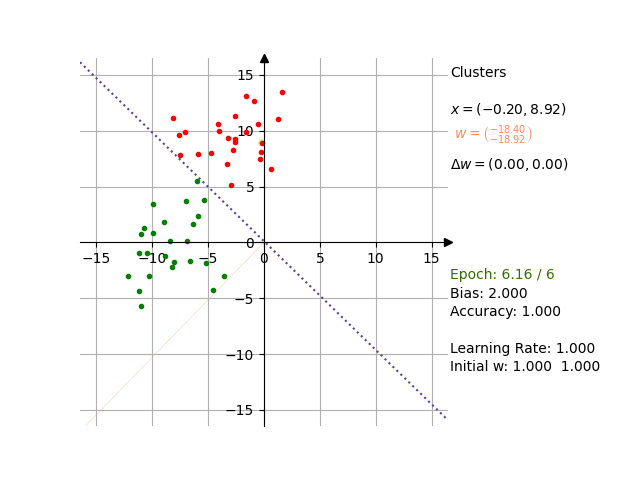
\includegraphics{images/rosenblatt/blob_success.png}
    \caption{Interpretationen der XOR-Funktion im kartesischen Koordinatensystem. Eine lineare Trenngerade existiert für die Werte nicht.}
    \label{fig-rp-xor}
\end{figure}

\subsection{Der KI-Winter}

In \textit{Perceptrons - An introduction to Computational Geometry (1969)} [MP17] behandeln \textit{Minsky und Papert} u.a. das Verhalten des Perzeptrons im Fall nicht-separabler Daten\footnotemark[35] sowie das Problem bzgl. \textit{recognition of connectedness}\footnotemark[36], bei dem es um die Erkennung zusammenhängender geometrischer Figuren geht.
Ihr Anliegen mit dem Buch ist es, die (mathematischen) Grenzen des Rosenblatt-Perzeptrons auf ein formales Gerüst zu stellen [MP17:249, ``What Perceptrons Can't Do``].
Ihre Ausführungen verstärken aber die ohnehin schon skeptische Haltung\footnotemark[37] gegenüber der Fähigkeiten des Perzeptrons\footnotemark[38] und künstlicher neuronaler Netze allgemein, was [AR88:159] rückblickend auch auf Aussagen in der Einleitung des Buches\footnotemark[39] zurückführen wie

\footnotetext[35]{
    in [MP17:181, ``11.8 The nonseparable case`` ff.]
}
\footnotetext[36]{
    [MP17:12, ``Theorem 0.8``],  _recognition of connectedness_ [MP17:249, letzter Abs. ff.]. In dem Epilog, der 19 Jahre später in einer Neuausgabe von _Minsky und Papert_ veröffentlicht wird, machen sie deutlich, dass sie damit nicht nachweisen wollten, dass ein Perzeptron nicht in der Lage zu der Erkennung zusammenhängender geometrischer Figuren sei, sondern dass die Komplexität von verschiedenen Aufgaben Anforderungen an ein Perzeptron stellt, die zu der damaligen Zeit (Ende 1950er / Anfang 1960er) schwierig umzusetzen gewesen sind [MP17:250, Abs. 2] &nbsp;
}
\footnotetext[37]{
    Here was a machine that could do pattern recognition in a humanlike way; it could recognize all kinds of things. Almost everyone at MIT was very skeptical`` [Cow98:99]
}
\footnotetext[38]{
    auch wegen schlechter Skalierbarkeit des Modells in der Praxis [AR88:159, Abs. 2]
}
\footnotetext[39]{
    [MP17,S. 1-20]
}

\blockquote[{[MP17:19. Abs. 3]}]{
hundreds of projects and experiments [bzgl. des Perzeptrons] were generally disappointing, and the explanations inconclusive. The machines usually work quite well on very simple problems but detoriate very rapidly as the tasks assigned to the get harder.
}

\noindent
Auch eine generelle Irritation und Enttäuschung über das Perzeptron-Modell meinen \textit{Anderson und Rosenfeld} zu erkennen:

\blockquote[{[MP17:232]}]{
we [Minsky und Papert] consider it to be an important research problem to elucidate (or reject) our intuitive judgement that the extension is sterile.
}

\noindent
Diesen ``Pessimismus`` betrachten \textit{Minsky und Papert} im Jahr 1988 in Retrospektive [MP17. S xxi]. Sie sind sich der Behauptung bewusst, ihr Buch hätte mit dem Aufzeigen der Grenzen des Rosenblatt-Modells den Forscherdrang an maschinellem Lernen gebremst:

\blockquote[{[MP17:xx]}]{
One popular version is  that the publication of our book so discouraged research on learning in network machines that a promising line of research was interrupted.
}

\noindent
In  [AR98:X] verweisen \textit{Anderson und Rosenfeld} auf [Cow90], in dem auch über ``the influence of Marvin Minsky and Seymour Papert on the loss of interest in neural networks during the 1970s`` [AR98:X] gesprochen wird.

\textit{Russell und Norvig} fassen zusammen, dass \textit{Minsky und Papert} in ihrem Buch bewiesen haben, dass ein Perzeptron alles lernen kann, was es auch darstellen kann, aber es könnte halt nur sehr wenig darstellen[RN09:45]\footnotemark[40]. Auf gleicher Seite verweisen sie auf die zunehmende Komplexität der zu berechnenden Modelle, die nicht alleine durch schnellere und bessere Hardware kompensiert werden konnte.

Der Lighthill Report\footnotemark[41] sollte dann 1973 eine Grundlage für die Entscheidung der britischen Regierung darstellen, das Budget für die Forschung an KI zu kürzen [RN09:45]. Neuronale Netze wurden als Grundlage künstlicher Intelligenz zunächst verworfen [Ola96:641, letzter Abs.], und die Forschung daran ging zurück, bis sie Anfang/Mitte der 1980er Jahre wieder aufgenommen wurde: Diese Periode ist gemeinhin als ``KI-Winter`` bekannt.


\footnotetext[40]{
vgl. hierzu [MP17:xxi, Abs. 1]
}
\footnotetext[41]{
``Workers entered the field around 1950, and even around 1960, with high hopes that are very far from having been realised in 1972. In no part of the field have the discoveries made so far produced the major impact that was then promised.`` in https://www.chilton-computing.org.uk/inf/literature/reports/lighthill\_report/p001.htm, ``3 Past disappointments``, abgerufen 28.08.2023
}
